\chapter{MDPs}

\section{MDP examples}\label{MDP-examples}

Here are some examples of MDPs in the wild.

\paragraph{Bus engine replacement}

\begin{itemize}
\tightlist
\item
  \textbf{States:} Accumulated mileage of each bus (since their last
  replacement).
\item
  \textbf{Actions:} Replace bus \(i\), Y / N. If Y, what year model to
  replace with?
\item
  \textbf{Transition fn:} How the mileage of each bus changes between
  fitness checks.
\item
  \textbf{Reward fn:} Age dependent recurring cost - for repairs - and
  replacement cost.
\end{itemize}

Note: The transition function could be diagonal, or not. If diagonal
then buses are not able to effect the milage of other busses, possibly
by taking another's shift. In this case, the problem is reduced to a
contextual bandit problem (?).

\cite{Putterman2015}

\hypertarget{the-aloha-protocol}{%
\paragraph{The ALOHA protocol}\label{the-aloha-protocol}}

\begin{itemize}
\tightlist
\item
  \textbf{States:} For each terminal, is last attempt a collision.
\item
  \textbf{Actions:} The probability of each terminal attempting to send
  a new packet (if there has been a collision).
\item
  \textbf{Transition fn:} Combines terminal packets into either a
  successful transmission, or a collision.
\item
  \textbf{Reward fn:} If a packet is sent, great. If not, bad.
\end{itemize}

\cite{Putterman2015} pg 8

\hypertarget{mate-desertion-in-coopers-hawks}{%
\paragraph{Mate desertion in Cooper's
Hawks}\label{mate-desertion-in-coopers-hawks}}

\begin{itemize}
\tightlist
\item
  \textbf{States:} The product of the brood's health and mother's health
  (\([2:7] \times [2:7]\)).
\item
  \textbf{Actions:} Stay, hunt, desert.
\item
  \textbf{Transition fn:} The four developmental stages, early nestling,
  late netling, early feldgling, late feldgling. From one developmental
  stage to the next, the energy levels of the mother and brood are
  determined by the initial energy reserves, the actions taken and the
  availability of food. (this was estimated from data data gatherd by
  \ldots{})
\item
  \textbf{Reward fn:}
\end{itemize}

\cite{Putterman2015} pg 10

\hypertarget{but-whos-counting}{%
\paragraph{But who's counting?}\label{but-whos-counting}}

\begin{itemize}
\tightlist
\item
  \textbf{States:} A random number, and the value of each of five
  possible locations. Possibly none value.
\item
  \textbf{Actions:} Choose which location to add the latest random
  number.
\item
  \textbf{Transition fn:} Deterministically updates the storage location
  given the action and observed random number.
\item
  \textbf{Reward fn:} The total magnitude of the stored number, only
  given after the storage is full..
\end{itemize}

\cite{Putterman2015} pg 13

\hypertarget{diagnosing-catnip-immunity}{%
\paragraph{Diagnosing catnip
immunity}\label{diagnosing-catnip-immunity}}

\begin{itemize}
\tightlist
\item
  \textbf{States:} The truth values for immuity to an of the 4 drugs (
  Catnip / Valerian / Silvervine / Honeysuckle )
\item
  \textbf{Actions:} Choose which drug to test.
\item
  \textbf{Transition fn:} Updates the truth values with some probability
  of returning a true postive or false negative.
\item
  \textbf{Reward fn:} Minimize the cost to find a working drug.
  Catnip=\$8.96, Valerian=\$7.00, Silverine=\$17.77, Honeysuckle=\$7.99.
\end{itemize}

\begin{quote}
Bol et al 2017, as noted, provides responses for 4 drugs
(catnip/Valerian/silvervine/honeysuckle) in a large sample of cats;
responses turn out to be heavily intercorrelated, permitting the ability
to better predict responses to the catnip alternatives based on a known
response to one of the others. This becomes useful if we treat it as a
drug selection problem where we would like to find at least one working
drug for a cat while saving money, and adapting our next test based on
failed previous tests.
\end{quote}

\begin{quote}
If they were not intercorrelated, one would simply minimize expected
loss in a greedy fashion, starting with catnip etc; but as they are
intercorrelated, now a drug has both direct value (if the cat responds)
and value of information (its failure gives evidence about what other
drugs that cat might respond to), which means the greedy policy may no
longer be the optimal policy.
\end{quote}

\href{https://www.gwern.net/Catnip\#optimal-catnip-alternative-selection-solving-the-mdp}{gwern
on Catnip}

This one is interesting. The four actions effect only the four state
element-wise. But our knowledge that certain immunities are correlated
make it possible to intelligently guess which tests should be performed.

\hypertarget{ad-targeting}{%
\paragraph{Ad targeting}\label{ad-targeting}}

\hypertarget{youtube-recommendation}{%
\paragraph{Youtube recommendation}\label{youtube-recommendation}}

\hypertarget{salamon-harvesting}{%
\paragraph{Salamon harvesting}\label{salamon-harvesting}}

\begin{itemize}
\tightlist
\item
  \textbf{States:} The size of the salamon population.
\item
  \textbf{Actions:} The size of the salamon population to be left to
  spawn.
\item
  \textbf{Transition fn:} Given the number left to spawn, it returns the
  size of the salamon population in the next season.
\item
  \textbf{Reward fn:} The size of salamon population harvested.
\end{itemize}

YOu might call this MDP a one dimensional MDP, as there is only a single
dimension that is acted up, is transitioned, is rewarded\ldots{} More
salamon

\href{http://www.it.uu.se/edu/course/homepage/aism/st11/MDPApplications1.pdf}{Real
applications of MDPs}

\hypertarget{fire-engine-allocation}{%
\paragraph{Fire engine allocation}\label{fire-engine-allocation}}

\begin{itemize}
\tightlist
\item
  \textbf{States:} The magnitude of a fire. The type of alarm. And the
  total number of first and second fire engines already deployed.
\item
  \textbf{Actions:} Whether to send more fire engines.
\item
  \textbf{Transition fn:} Given the number of fire engines fighting the
  fire, and the fires type / magnitude, the building may be destroyed or
  saved. Fire may start at anytime, in a random location throughout the
  city.
\item
  \textbf{Reward fn:} Damage incurred by the fires.
\end{itemize}

\href{http://www.it.uu.se/edu/course/homepage/aism/st11/MDPApplications1.pdf}{Real
applications of MDPs}

Other possible MDPs?

\begin{itemize}
\tightlist
\item
  An animal stockpiling food?!
\item
  Robotics / movement
\end{itemize}

\begin{center}\rule{0.5\linewidth}{\linethickness}\end{center}

More Refs

\begin{itemize}
\tightlist
\item
  http://www.it.uu.se/edu/course/homepage/aism/st11/MDPApplications1.pdf
\item
  https://www.worldscientific.com/worldscibooks/10.1142/p809
\end{itemize}

\section{Tabular MDPs}\label{vf-neumann}

It is possible to derive the value functional in another, possibly more enligtening way. But it takes a little more work. It requires a result from real analysis, the Neuman series. Which is simply the generalisation of a geometric series to contractive linear operators, such as a matrix.

\begin{align*}
r &\in (-1, 1) \\
(1-r)^{-1} &= \lim_{n\to \infty} \sum_{i=0}^n r^i \tag{Geometric series}\\
T &\in \mathbb X^k: \det(T) \in (-1, 1) \\
(I-T)^{-1} &= \lim_{n\to \infty} \sum_{i=0}^n T^i \label{eq:neumann}\tag{Neumann series}
\end{align*}

We can expand the recursion in the Bellman equation to get an \eqref{eq:inf-series}. We can then use the \eqref{eq:neumann} (by setting $T=\gamma P_{\pi}$) to give the nice analytic form of the value functional.

\begin{align*}
V &= r_{\pi} + \gamma P_{\pi} V \tag{Bellman eqn}\\
V &= r_{\pi} + \gamma P_{\pi}\big( r_{\pi} + \gamma P_{\pi} V\big) \\
V &= r_{\pi} + \gamma P_{\pi}\Big(r_{\pi} + \gamma P_{\pi}\big( r_{\pi} + \gamma P_{\pi} V\big)) \\
&= r_{\pi} + \gamma P_{\pi}r_\pi + \gamma^2 P_{\pi}P_{\pi}r_{\pi} + \gamma^3 P_{\pi}P_{\pi}P_{\pi}V \\
&= \sum_{t=0}^{\infty} \gamma^tP_{\pi}^tr_{\pi} \label{eq:inf-series}\tag{infinite series} \\
&= \big( \sum_{t=0}^{\infty} \gamma^tP_{\pi}^t \big) \cdot r_{\pi}\\
&= (I-\gamma P_{\pi})^{-1} r_{\pi} \tag{value functional}\\
\end{align*}

This proof is more satisfying because we can more clearly see the nature of the value functional. It is a closed form of the infinite sum of discounted future rewards.


\section{Policies in high dimensions}\label{high-D-policies}

Let's \textit{try} to gain some intuition about the space of policies in higher dimensions.
For each state, we have a distribution (on a simplex), over the possible actions.

\begin{figure}[h]
\centering
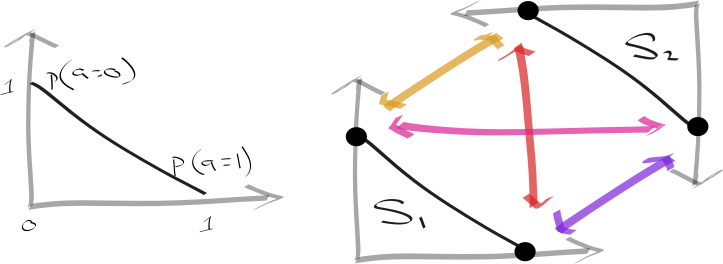
\includegraphics[width=1\textwidth,height=0.20\textheight]{../../pictures/drawings/2-state-2-action-simplices.png}
\caption{Imagine what the geometry of the space of policies in the two state, two action MDP. A policy tells us what actions should be taken when in a given state. Therefore, there will be \(|A| \times |S|\) entries in the policy. However, because the policy returns a distribution over actions, the true dimensionality of the policy is \((|A| -1) \times |S|\). Which in the two state, two action case equals 2D.}
\end{figure}

\begin{figure}[h]
\centering
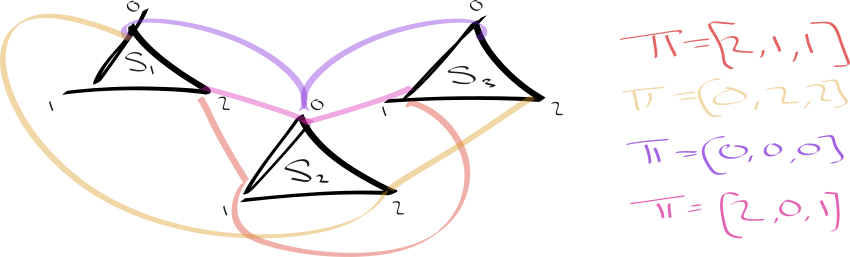
\includegraphics[width=1\textwidth,height=0.25\textheight]{../../pictures/drawings/3-state-3-action-simplices.png}
\caption{Here we are visualising the policy space of a three state, three action, MDP.
For each state, we must specify a distribution over actions.}
\end{figure}

\newpage

\section{Other properties of the polytope} \label{polytope-extras}



\subsection{Distribution of policies}

A potentially interesting question to ask about the value polytope is how the
values (of the policies) are distributed. To calculate this
analytically, we can use the probability chain rule:
\(p(f(x)) = \mid \det\frac{\partial f(x)}{\partial x}\mid^{-1}p(x)\).
Where we set \(f\) to be our value functional and \(p(x)\) to be a
uniform distribution over policies. Thus we have;

\begin{align}
p(V(\pi)) = |\det \frac{\partial V(\pi)}{\partial \pi}|^{-1} \cdot p(\pi) \tag{density}
\end{align}

\begin{figure}
\centering
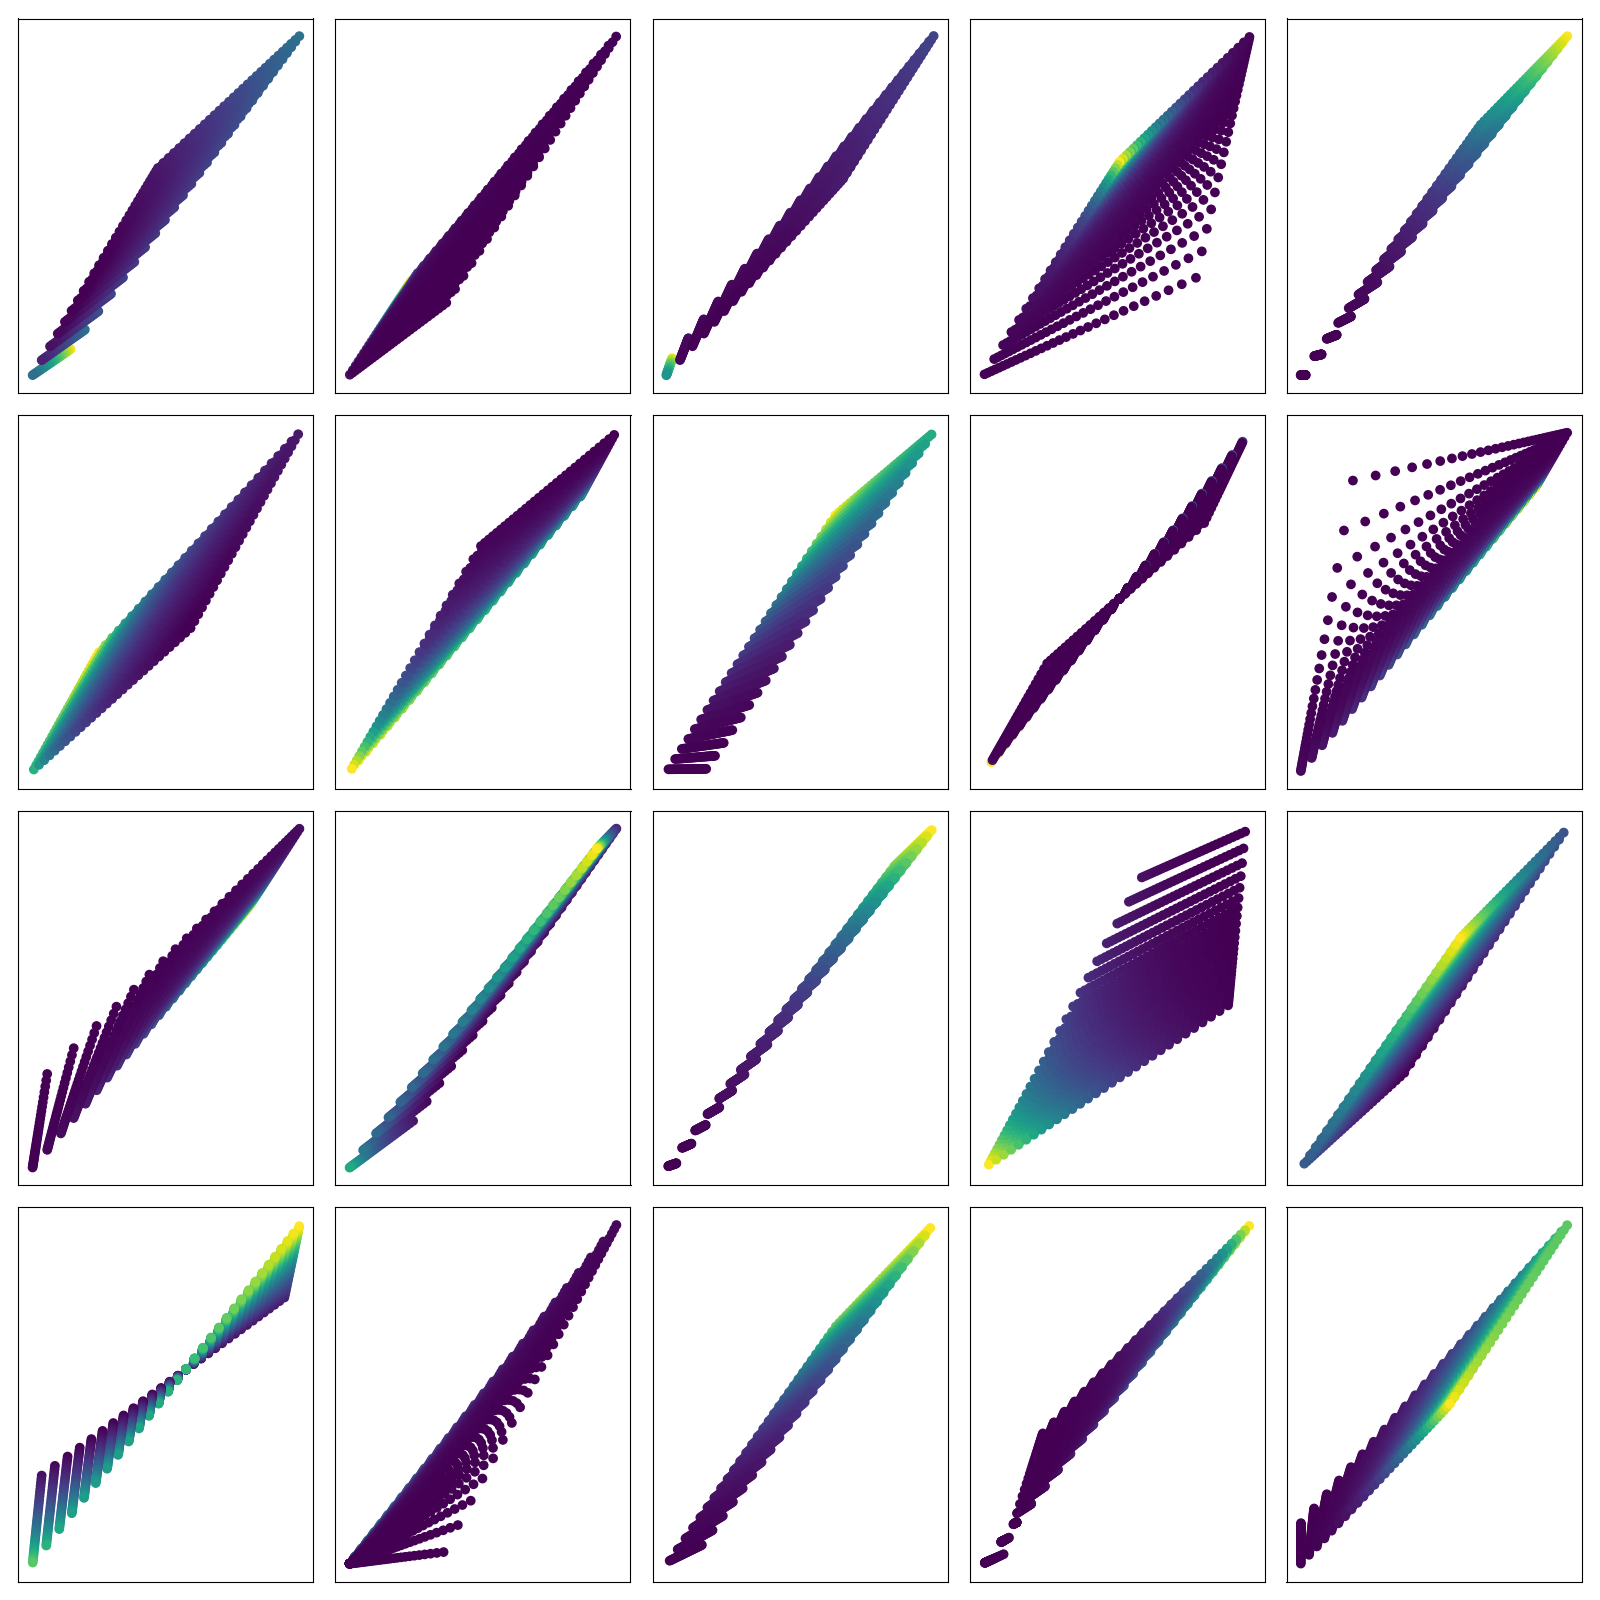
\includegraphics[width=1\textwidth,height=1\textheight]{../../pictures/figures/polytope_densities.png}
\caption{2-state 2-action MDPs. We have visualised the likelihood of
values under a uniform distribution over policies. They are coloured by density.
Lighter colour is higher probability.}
\label{fig:density}
\end{figure}

We can see in \ref{fig:density}, that in some polytopes, many of the policies are close
to the optimal policy. In other polytopes, many of the policies are far
away from the optimal policy. Does having many policies that have close to
optimal value make the MDP easier to solve?

{\color{red}Finish this off!? Would be good to show that a there exist 'easily solvable'
 MDPs. But your chance of getting one is effectively zero}

\subsubsection{An MDPs Entropy}

{\color{red}not sure where this is going...}

We can visualise polytopes in 2D, but we struggle in higher dimensions.
However, it is possible to use lower dimensions to gain intuition about
metrics and carry that intuition into higher dimensions. A potential
metric of interest here is the entropy of our distribution, (and / or
the expected distance from the optima) to give intuition about
unimaginable MDPs.

\begin{align}
M &\to \{P, r, \gamma\} \tag{a MDP}\\
H(M) &:= \mathop{\mathbb E}_{\pi\sim\Pi}\Big[-\log p(V(\pi)) \Big]\\
&= \mathop{\mathbb E}_{\pi\sim\Pi}\Big[-\log(\mid \det\frac{\partial V(\pi)}{\partial \pi}\mid^{-1}p(\pi)) \Big] \\
&= \mathop{\mathbb E}_{\pi\sim\Pi}\Big[-\log(\mid \det \frac{r}{(I-\gamma P \pi)^2}\mid^{-1}p(\pi)) \Big] \\
\end{align}

What does this tell us? \textbf{???} A MDP with a low entropy tells us
that many of the policies are in a corner of the polytope. But the
`hardness' of the MDP depends on which corner these policies are
concentrated in. Rather we could use the value of each policy to give
information about the location of the policy.

\begin{align*}
\mu(M) &:= \mathop{\mathbb E}_{\pi\sim\Pi}\Big[V(\pi) \Big]\\
\end{align*}

What does this tell us? The expected value of a policy. Thus, a quantity
of interest might be the expected suboptimality of a policy,
\(s = V(\pi^{* })-\mu(M)\). This tells us how far away the optimal
policy is from the center of mass of the polytope.

\textbf{Conjecture:} If an MDP has suboptimality
\(s \le \frac{\sigma_{MDP}}{D}\) then it is possible to find a
\(\epsilon\) optimal policy with \(\mathcal O(n)\) samples. (but
sampling in high dimensions always scales badly?!)

\textbf{Experiment:} Correlate the properties of \(P, r\) with entropy.
Or find derivative wrt \(P, r\). What properties of \(P, r\) yield
easily solvable MDPs?

\subsection{Discounting}

Another question you may have is: \textit{how does the shape of the polytope depend on the discount rate?}
Given an MDP, we can vary the discount rate from \(0\) to \(1\) and visualise
the shape of the value polytope. Seen in \ref{fig:polytope-discounts}.

\begin{figure}
\centering
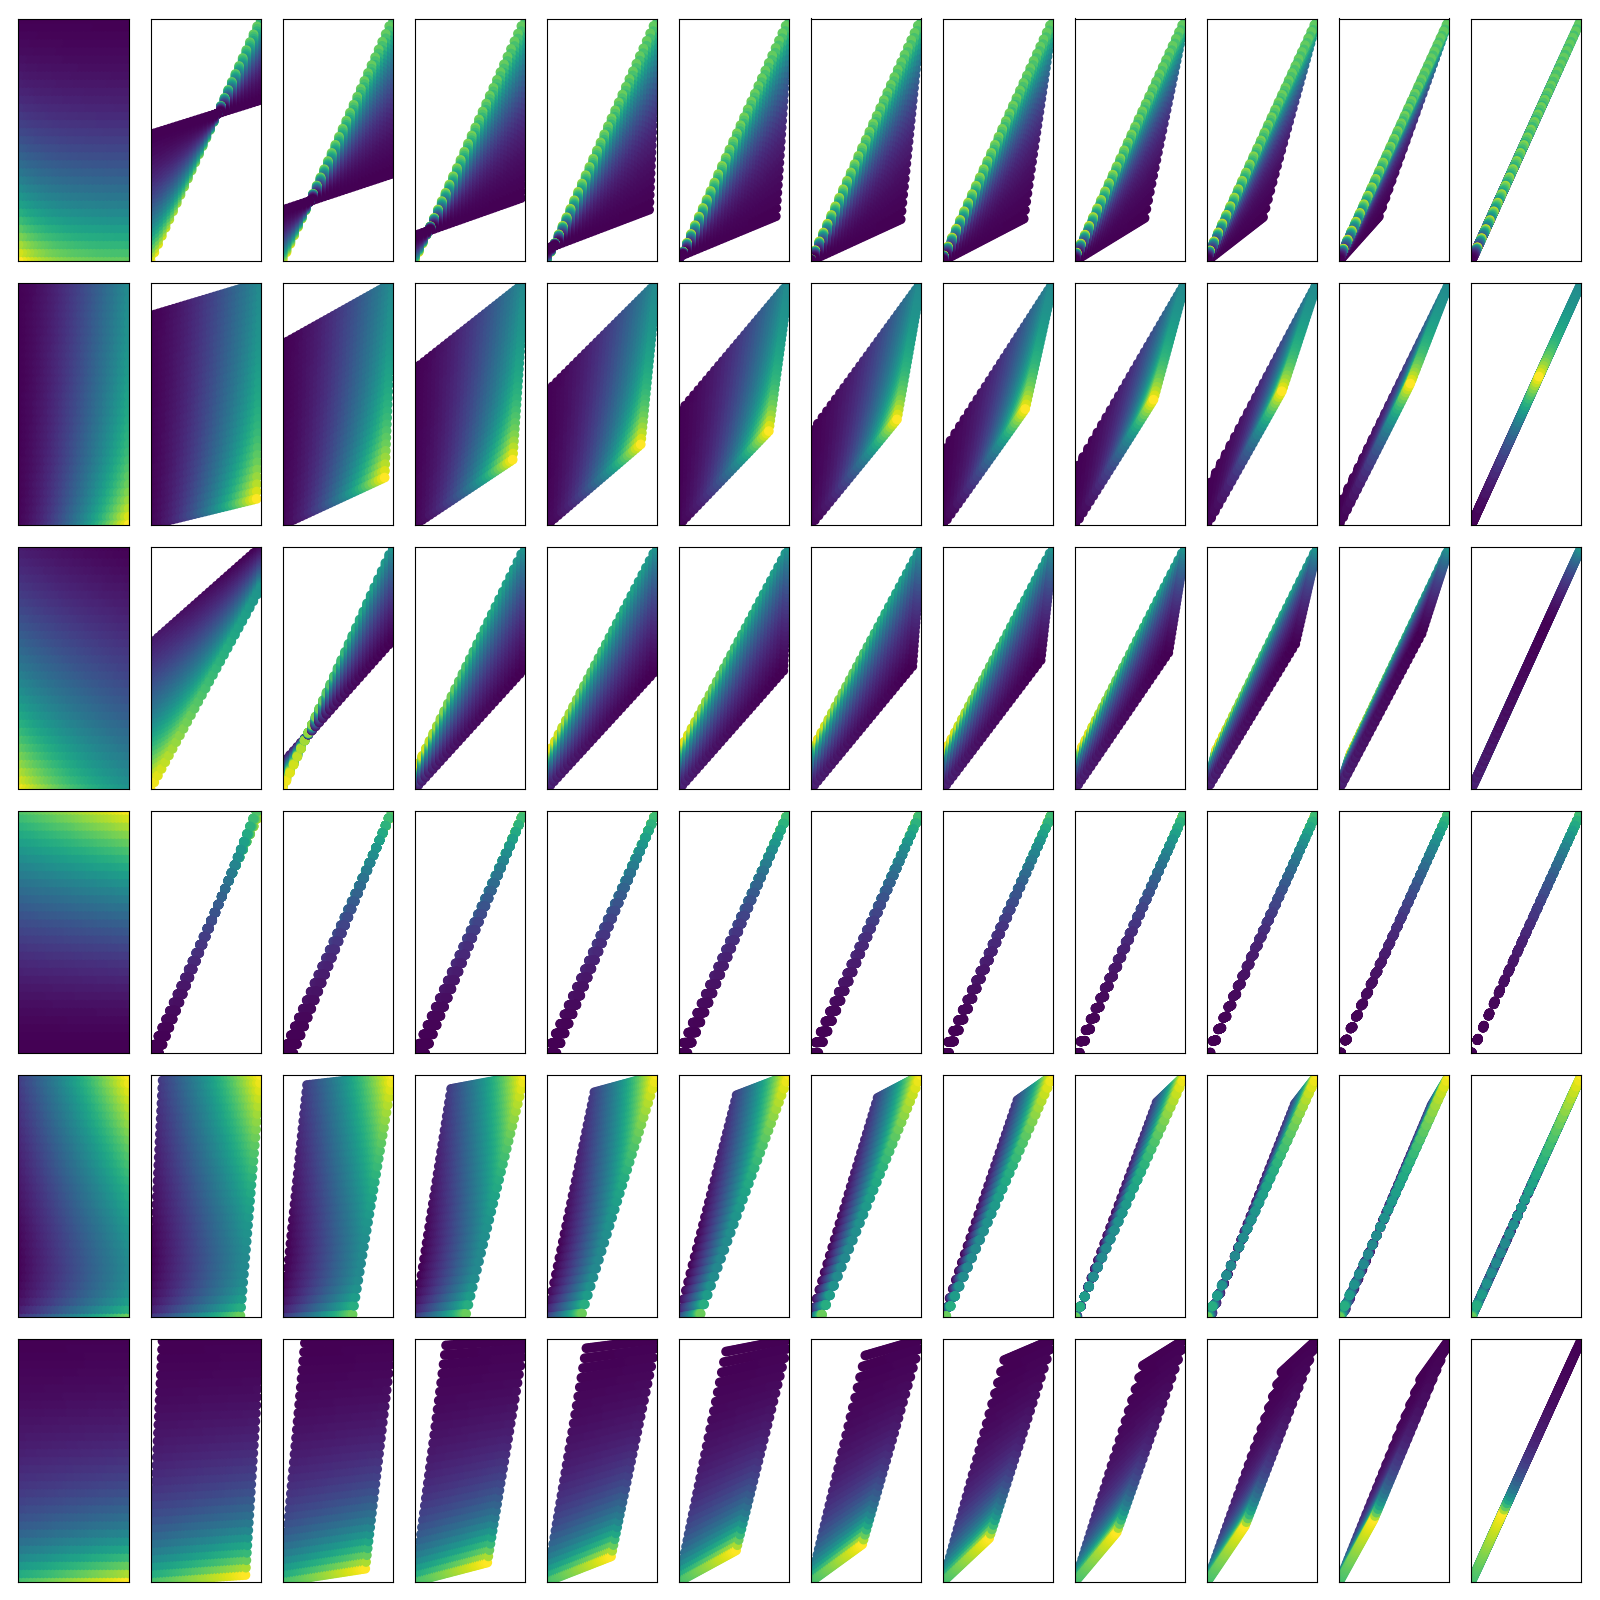
\includegraphics[width=1\textwidth,height=1\textheight]{../../pictures/figures/discounts.png}
\caption{Here we have shown a few different 2 state, 2 action, MDPs and how
their polytopes change with changes in discount rate, ranging from 0 (left), to 1 (right).
The color map is represents the density of policies, as in \ref{fig:density}.}
\label{fig:polytope-discounts}
\end{figure}

\begin{itemize}
\item
  \textbf{Observation} As \(\gamma \to 1\), all the policies are
  projected into a 1D space? \textbf{Question} Does this make things
  easier to learn? \textbf{Intuition} Orderd 1D spaces are easy to
  search.
\item
  \textbf{Observation} The tranformation that changing the discount
  applies is quite restricted. They are not generally non-linear, but
  appear `close to linear', but not quite. \textbf{Question} What is the
  set of functions /transformations that the discount can apply?
\end{itemize}

{\color{red}Finish this off!? Would be good to show that as discount tends to 1 then polytope collapses to a line?!?}

\subsection{Derivation of derivative}

\begin{align*}
V(\pi) &= (I − \gamma P_{\pi})^{−1}r_{\pi} \tag{value functional}\\
&= (I − \gamma P\cdot \pi)^{−1}r\cdot \pi \\
\frac{\partial V}{\partial \pi} &= \frac{\partial}{\partial \pi}((I-\gamma P_{\pi})^{-1} r_{\pi}) \\
&= (I-\gamma \pi P)^{-1} \frac{\partial \pi r}{\partial \pi}+   \frac{\partial (I-\gamma \pi P)^{-1}}{\partial \pi}\pi r\tag{product rule} \\
&= (I-\gamma \pi P)^{-1} r + -(I-\gamma \pi P)^{-2} \cdot -\gamma P\cdot \pi r\\
&= \frac{r}{I-\gamma \pi P} + \frac{ \gamma P\cdot \pi r}{(I-\gamma \pi P)^2} \tag{rewrite as fractions}\\
&= \frac{r(I-\gamma \pi P) + \gamma P \pi r}{(I-\gamma \pi P)^2} \tag{common demoninator}\\
& = \frac{r}{(I-\gamma P \pi)^2} \tag{cancel}
\end{align*}

TODO. Annotate. Add numbers and explain.



\section{Model search} \label{model-iteration}

As noted in \ref{search-spaces-mdps}, we can search through policy space or value
space when trying to solve a MDP. There is a third search space ...???



Lastly, we can search through possible models, $P, r$. Models that fit the
observations we make. That is policy $\pi_i$ has a value $V^{\pi_i}$.

\begin{displayquote}
  \textit{This model predicts that the ??? policy is of high value.
  However, when I tried this policy, I ended up with ...?
  My model must be wrong.}
\end{displayquote}

Here the parameters are composed to two independent parts, the transition function
and the reward function.

\begin{align}
\tilde P^{* }, \tilde r^{* } = \mathop{\text{argmin}}_{\tilde P, \tilde r} \int_{\Pi} \parallel V^{\pi}_{P, r} -V^{\pi}_{\tilde P, \tilde r} \parallel_\infty
\end{align}

While it is nice to have $\tilde P^{* }, \tilde r^{* }$, the ultimate goal of
solving a MDP is to find the optimal policy. ...!?!?

\subsection{Relationship to model based RL}

Most model-based learning approaches to RL ... next step prediction (refs!!!)
This algorithm only focuses on relevant features of the state space.

Consider a problem where the reward is only determined by the first feature of the state. We can add $n$ extra, useless, features.
The model based learner will spend resources on attempting to build a good predictor of those $n$ features.

Sample efficient. You only need to collect data for the $m$ policies we are matching under.
Once that has been done, the optimisation problem is easily solved!?

Model iteration. Model invariant transforms. Pick a policy. Falsify it,
and this falsify all models that yield the same optimal policy.

\begin{figure}[!h]
\centering
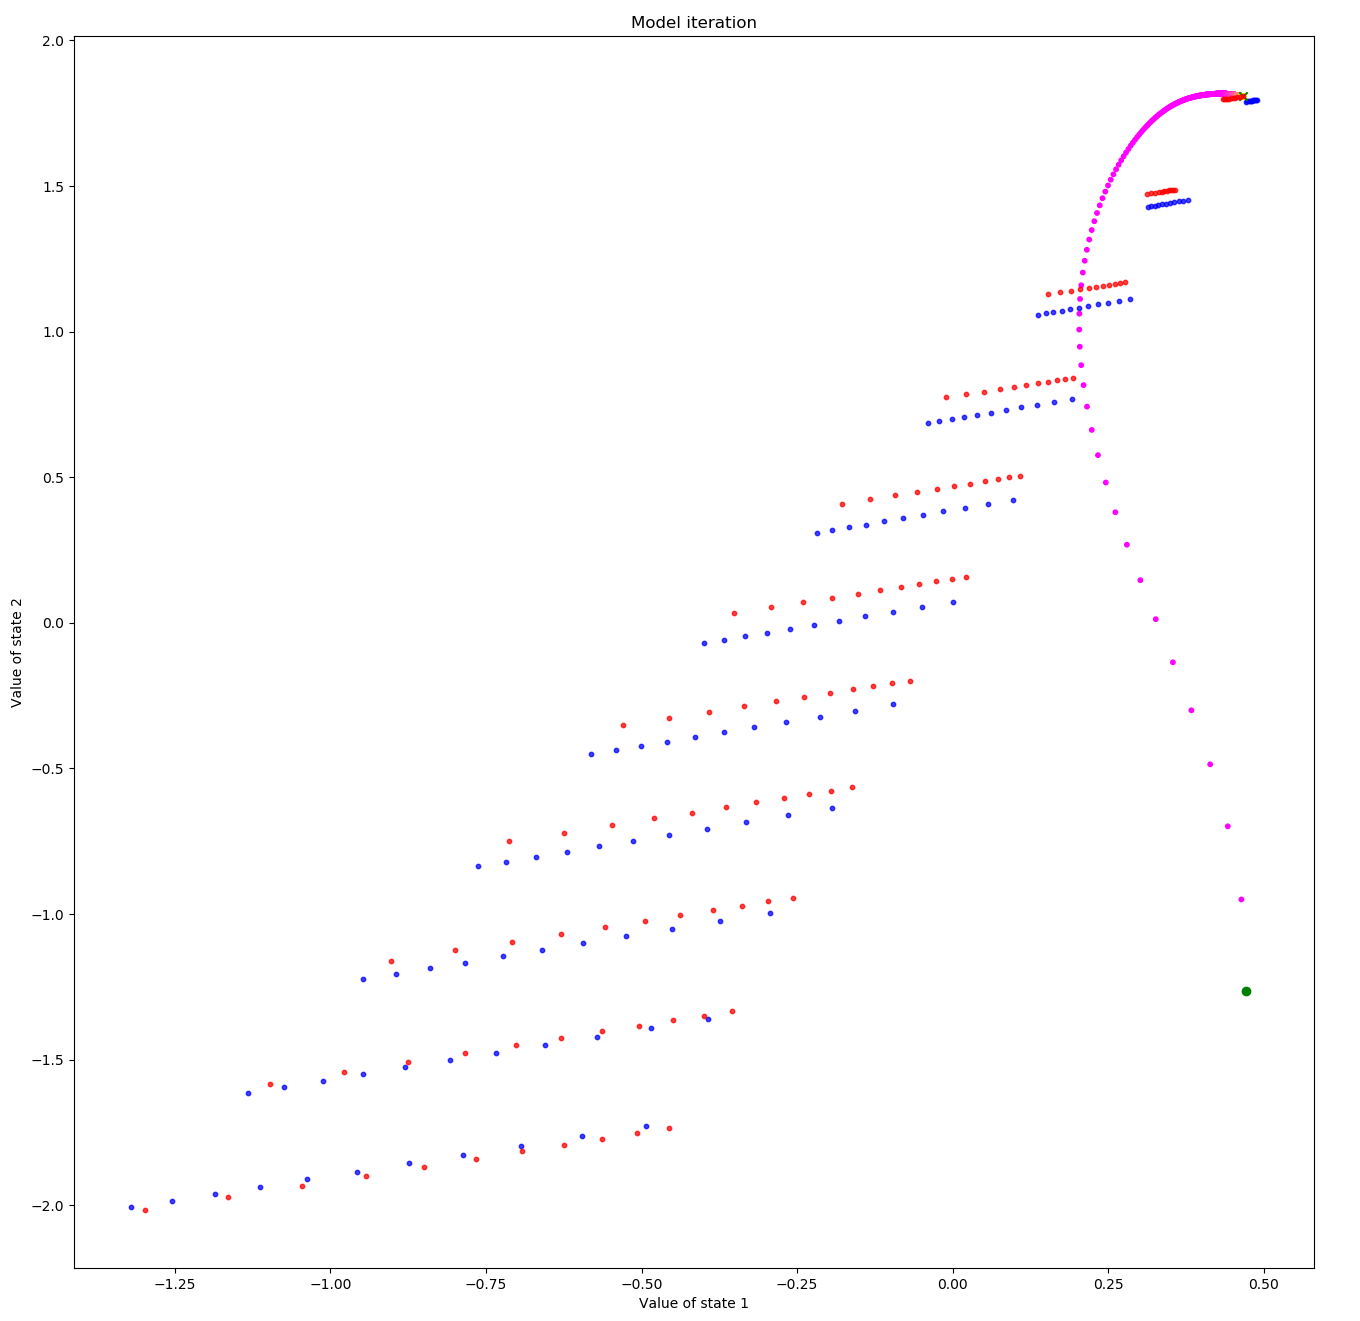
\includegraphics[width=0.35\textwidth,height=0.35\textheight]{../../pictures/figures/model_iteration.png}
\caption{Blue shows the value of policies when evaluated under the true model, $P, r$,
and Red shows the estimated value of policies when evaluated under the learned model at convergence, $\tilde P, \tilde r$.}
\end{figure}


Related to AWR? https://arxiv.org/pdf/1910.00177.pdf



\section{Visualising higher dimensional MDPs}\label{graph-vis}

So this value polytope works well for 2D. And could be extended to 3D. But, what about higher dimensions?

\begin{displayquote}
  \textit{"To deal with a 14-dimensional space, visualize a 3-D space and say 'fourteen' to yourself very loudly. Everyone does it."} Geoff Hinton
\end{displayquote}

Is there intuition we might gain from visualising optimisation on MDPs with the
number of states and / or actions being greater than 3?

How to construct them? Decompose the value of a policy as a convex combination
of the values of the deterministic policies.

\begin{align*}
  \alpha(\pi) = \mathop{\text{argmin}}_{\alpha \in \Delta^n} \parallel  V(\pi) - \sum_i (V(\pi_i) \cdot \alpha_i ) \parallel_2^2 + H(\alpha)
\end{align*}

The entropy term ensures we prefer convex combinations with lower entropy, (in this case, aka higher sparsity).

Properties of the graphs / graph signals?

\begin{figure}[!h]
\centering
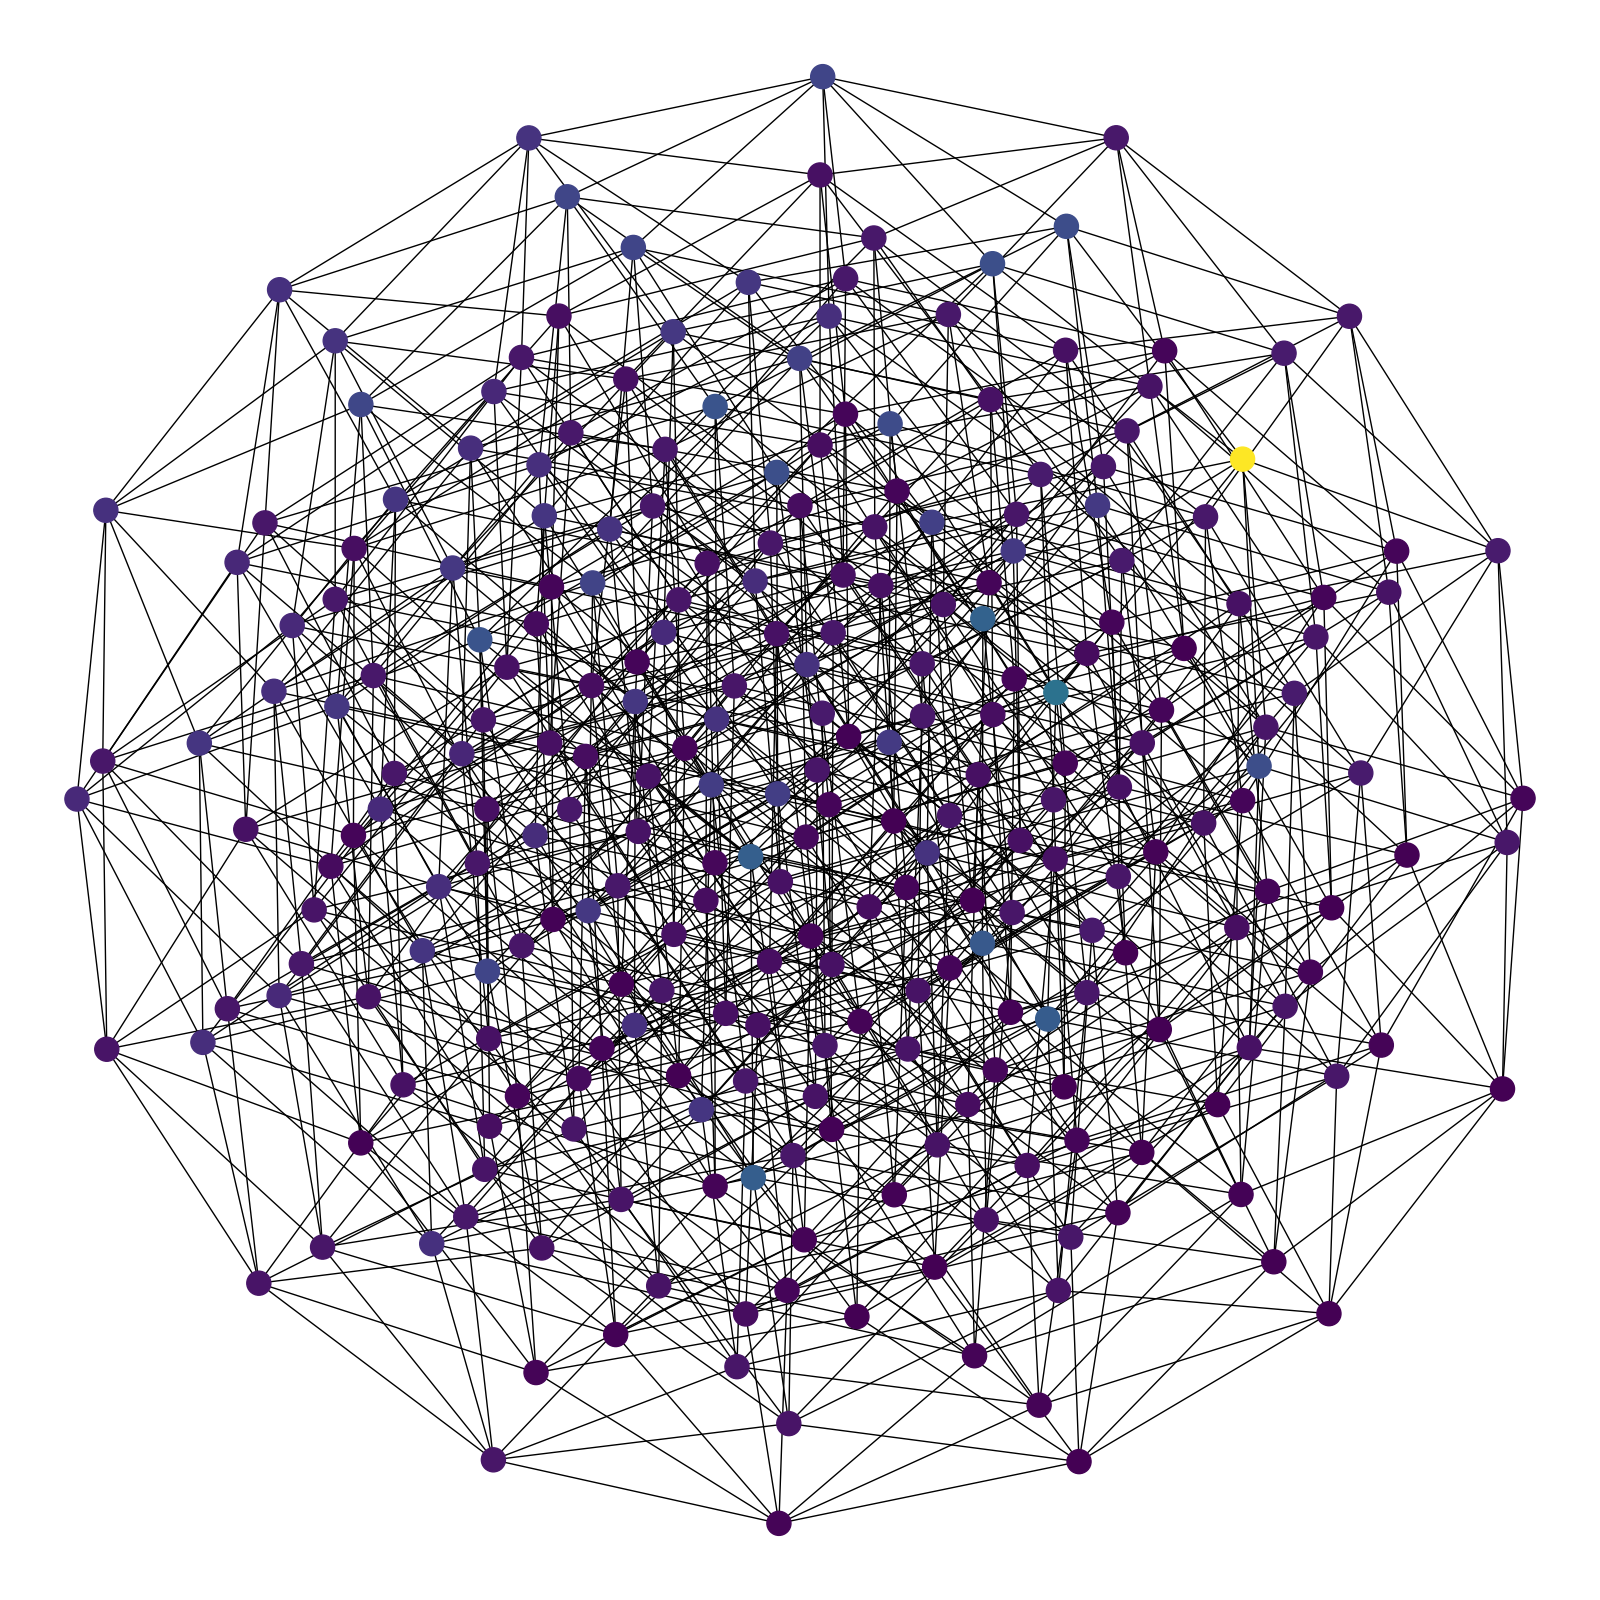
\includegraphics[width=0.5\textwidth,height=0.3\textheight]{../../pictures/figures/discrete-graph.png}
\caption{Policy iteration bounces between the nodes of the graph. As each node is a deterministic policy.
Thus policy iteration is equivalent to finding the shortest path on a XX connected policy graph. }
\end{figure}

{\color{red} wanta better picture}

\begin{figure}[!h]
\centering
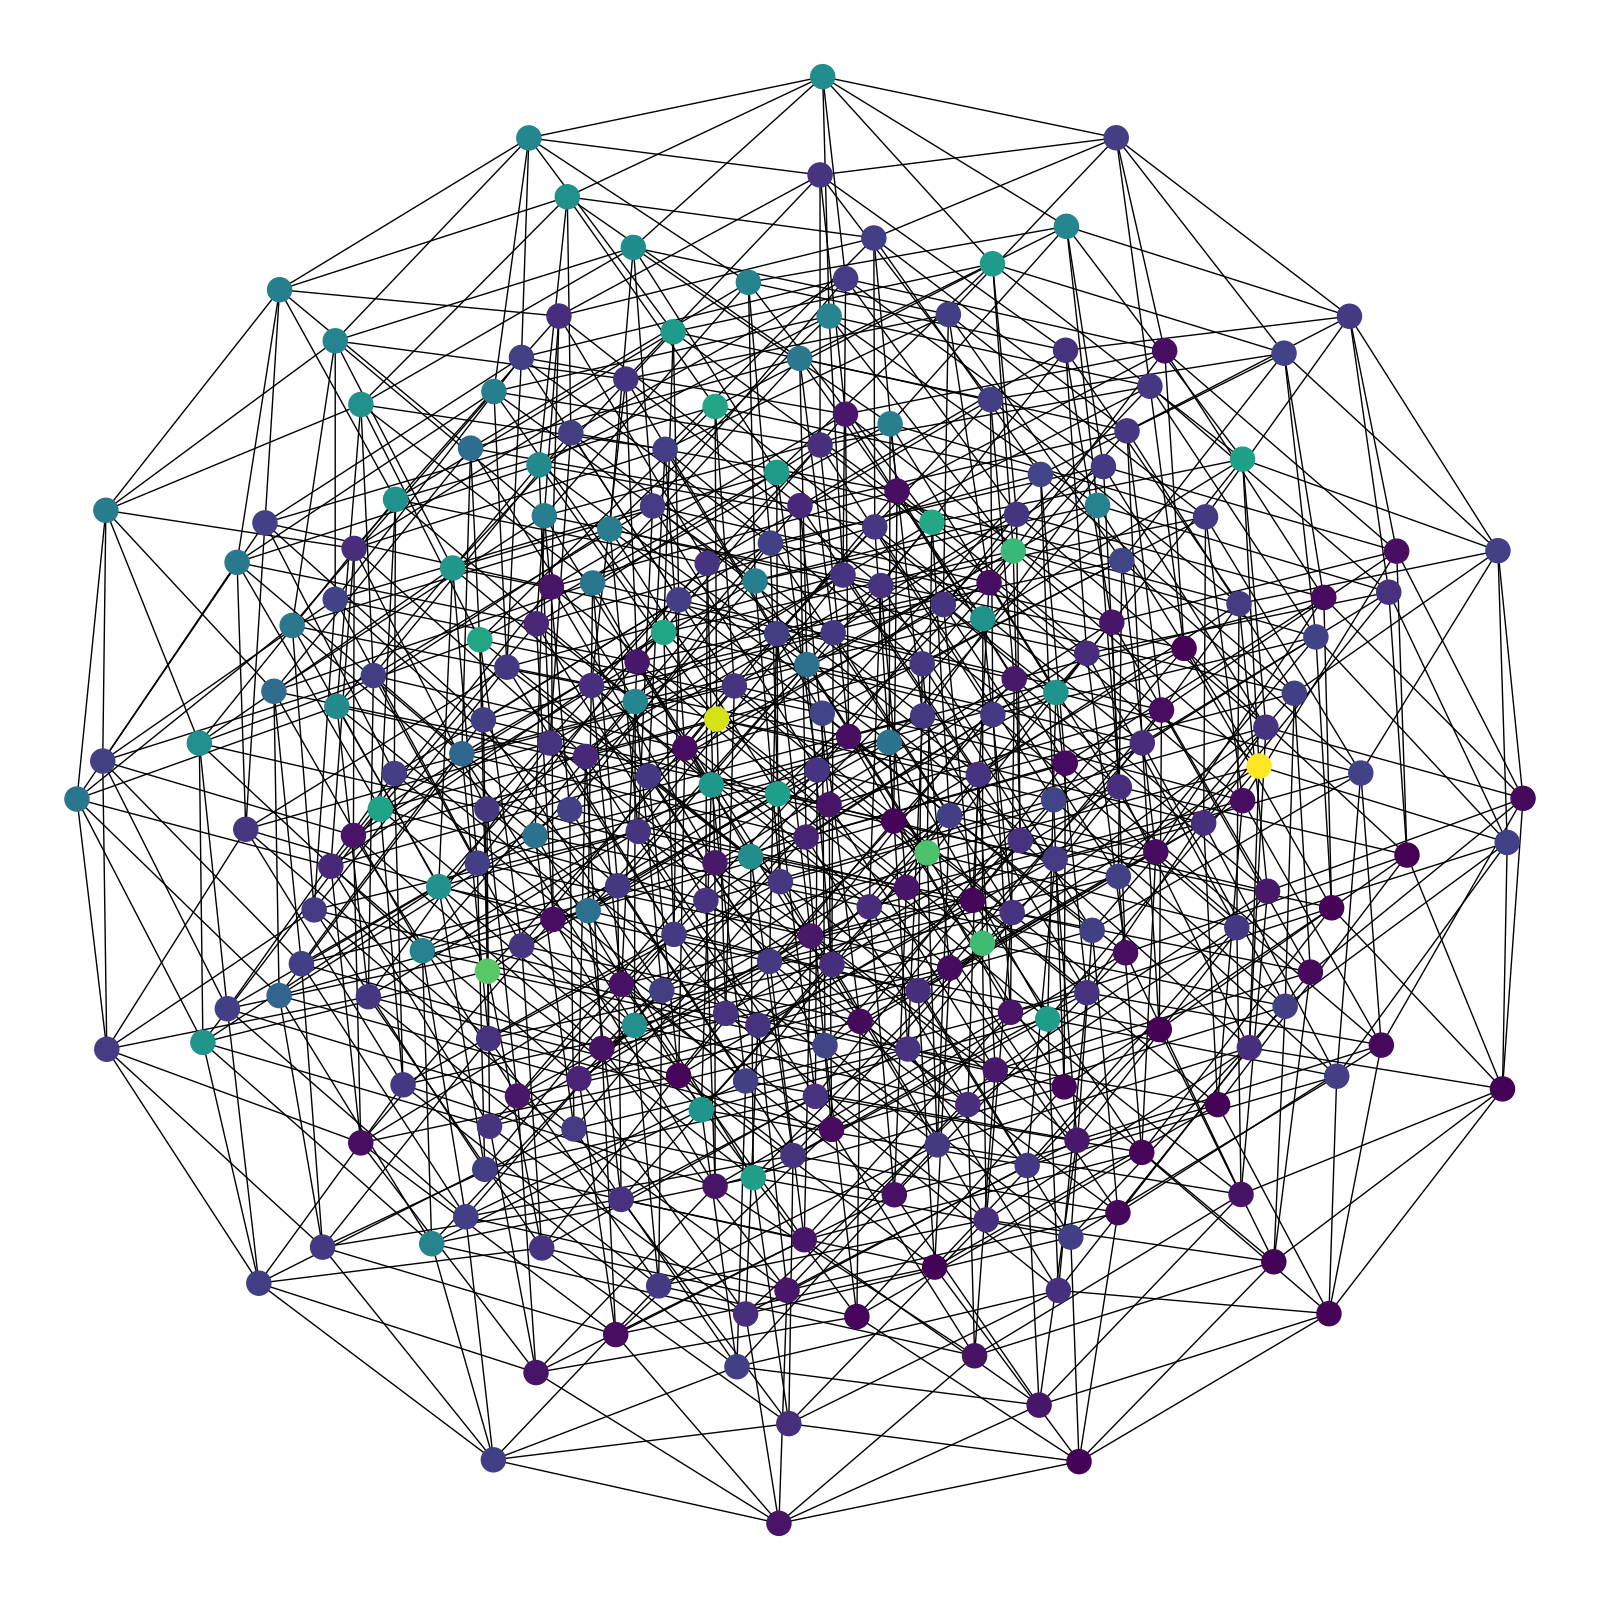
\includegraphics[width=0.5\textwidth,height=0.3\textheight]{../../pictures/figures/interior-graph.png}
\caption{Policy gradient traverses through non-deterministic policies, thus we can visualise how
close the current policy is to deterministic ones.}
\end{figure}


\section{Deep policy gradients}\label{ss-extras}

Currently, the most successful RL solvers are a variant of policy gradient methods \cite{Mnih2016,Schulmanb}.
And are being combined with deep parameterised models. (refs)
We would like to understand how parameterisation and policy gradients ...?

% In which spaces can we get the most information? (e.g. low variance gradients)
% In which spaces to we have access to reliable guidance (e.g. large magnitude gradients)?
% SNR

Overparam. DL. \cite{Arora2018}

Ok. So when $\phi$ are the parameters of a deep neural network, ...? The search space has certain (which) properties.
Euclidean geometry.
(parameter dimensions are independent! no funny business)

We can pick any space we we like to search with in. But, why would we want to pick one space over another?
What properties are we looking for?

\begin{figure}[!h]
\centering
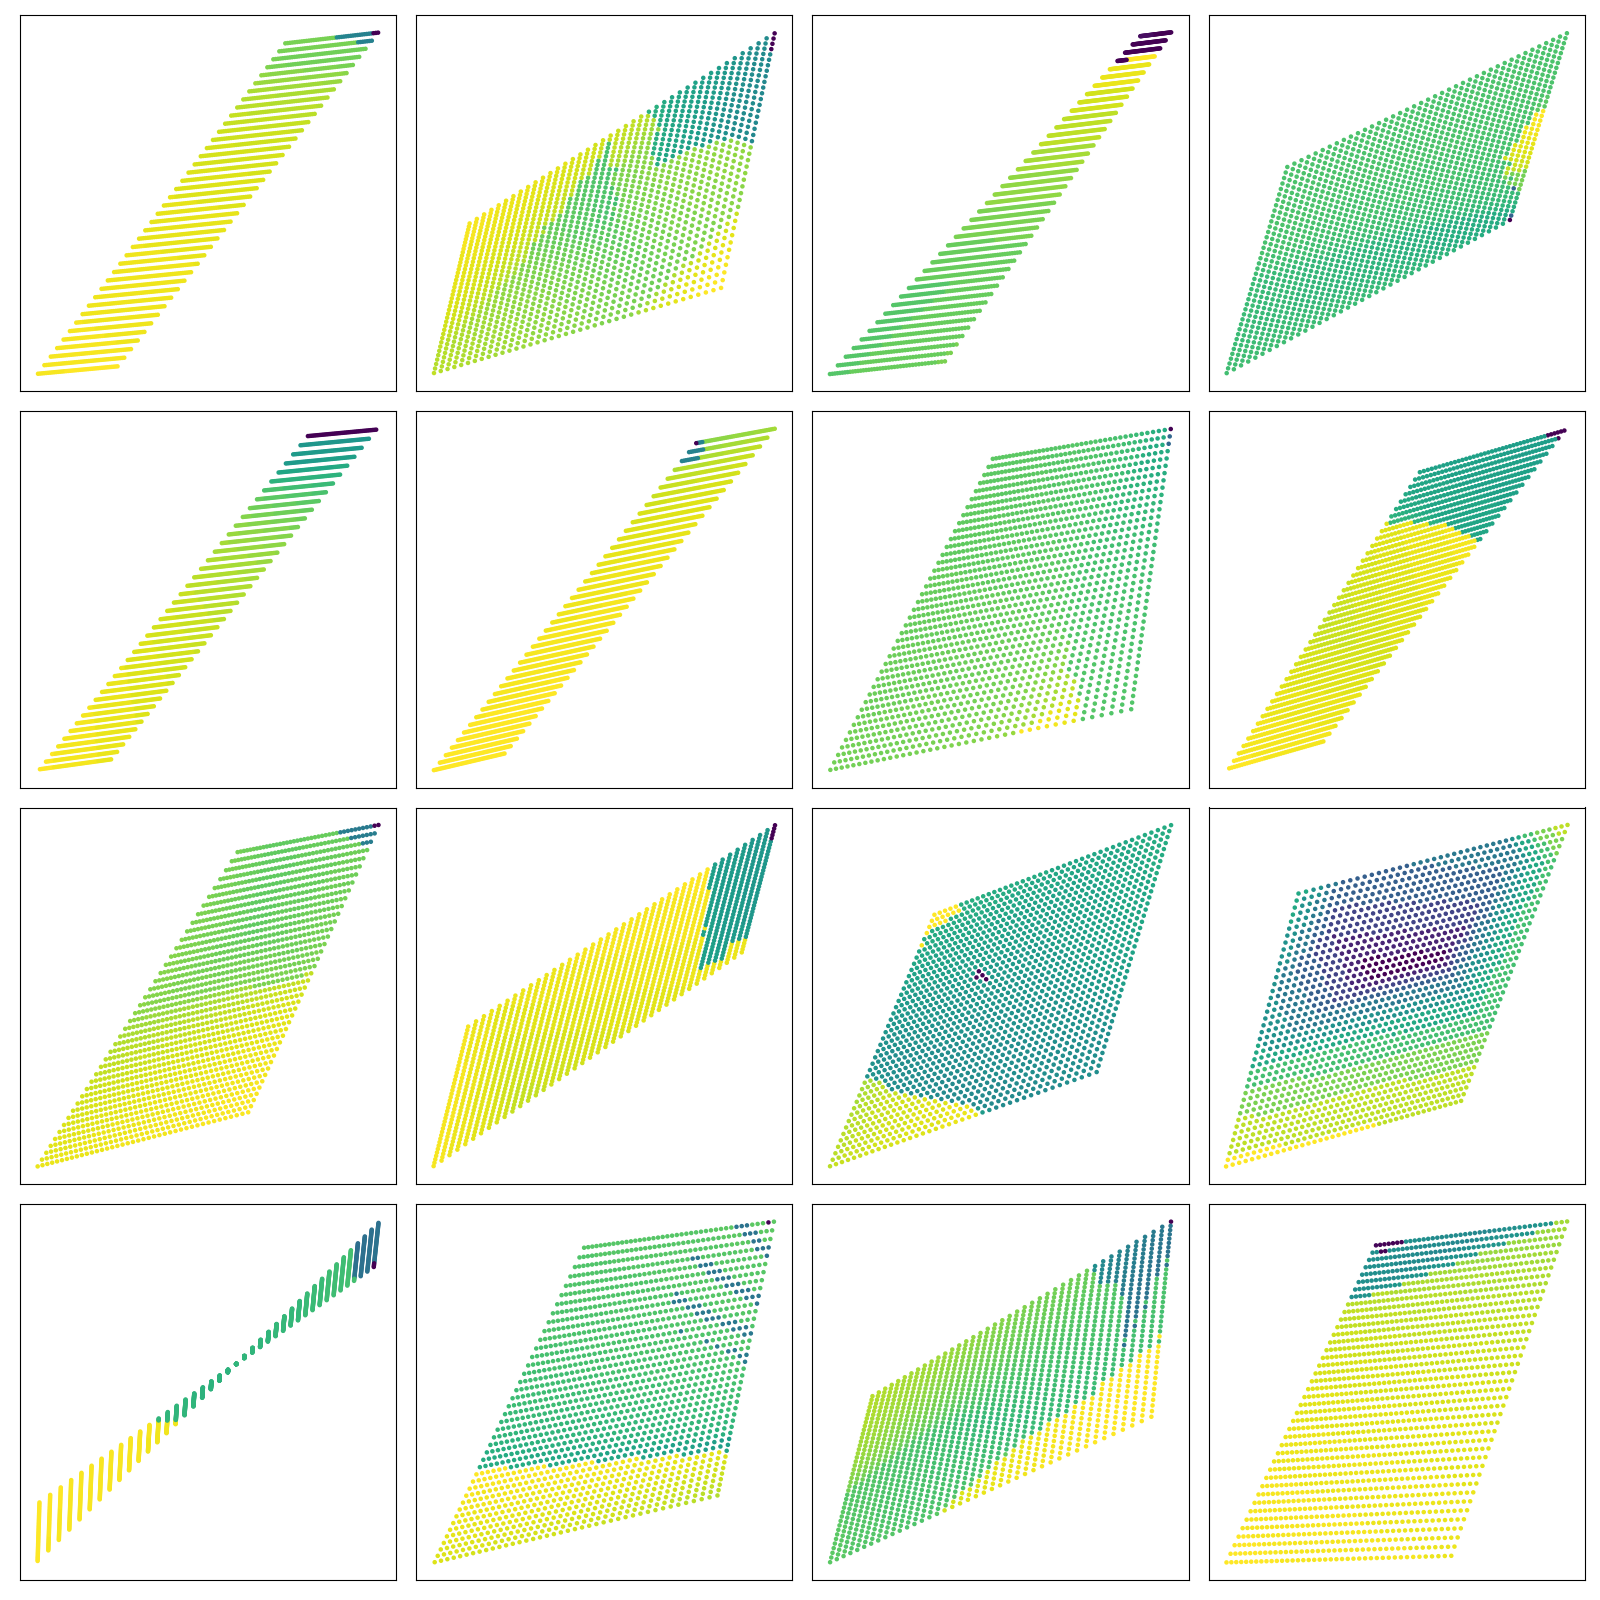
\includegraphics[width=1\textwidth,height=1\textheight]{../../pictures/figures/mvi-iterations.png}
\caption{Above you see: various MDPs where the value of each policy is colored
by the number of iterations it took to converge to the optimum policy. Yellow is many iterations, purple is few iterations.}
\end{figure}

\begin{itemize}
\tightlist
\item In which spaces can we (efficiently) calculate gradients?
\item In which spaces can we do convex optimisation?
\item In which spaces does momentum work (well)?
\end{itemize}


\begin{itemize}
\tightlist
\item
  What are the best ways to travel through policy space? (lines of
  shortest distance?!)
\item
  How does this scale with \texttt{n\_actions} or \texttt{n\_states}??
\item
  Is there a way to use an interior search to give info about the
  exterior? (dual methods?!)
\item
  What if your evaluations are only \(\epsilon\)-accurate? How does that
  effect things?!?
\item
  how can we pick the topology for better dynamics!?
\end{itemize}

\section{Topology and dynamics}

\cite{Tsitsiklis2000} linear value iteration converges. When linear means ... . But we consider linear value function of the form ...
Which diverge.

\cite{Brandfonbrener2019} consider the same setting, with an additional simplification. In the cts limit. No step sizes / learning rate.
Obviously this simplification is not realistic. As in our experiments we see divergence with a overparameterised linear model.

What kinds of query and movement does our search space support?

If we parameterise our search space. We my have changed the topology of our search space.
Is it possible to arbitrarily change the topology? (probably?!?)

\textbf{Q:} How can we rationally pick the topology of our search space
to accelerate learning?
Aka how can we pick function classes (function approximators) that support the bellman equation?

\begin{itemize}
\item
  A well connected space? For all possible policies, there exists
  \(\theta_1, \theta_2 \text{ s.t. } \parallel \theta_1- \theta_2\parallel_2\)
  is small. (but that doesnt necessarily help\ldots{} depends on the
  landscapce imposed by \(\nabla_{\theta} V\))
\item
  ???
\end{itemize}

See these gradient flows for example;

Pics?!?

Here are some examples \ldots{}???

\begin{figure}
\centering
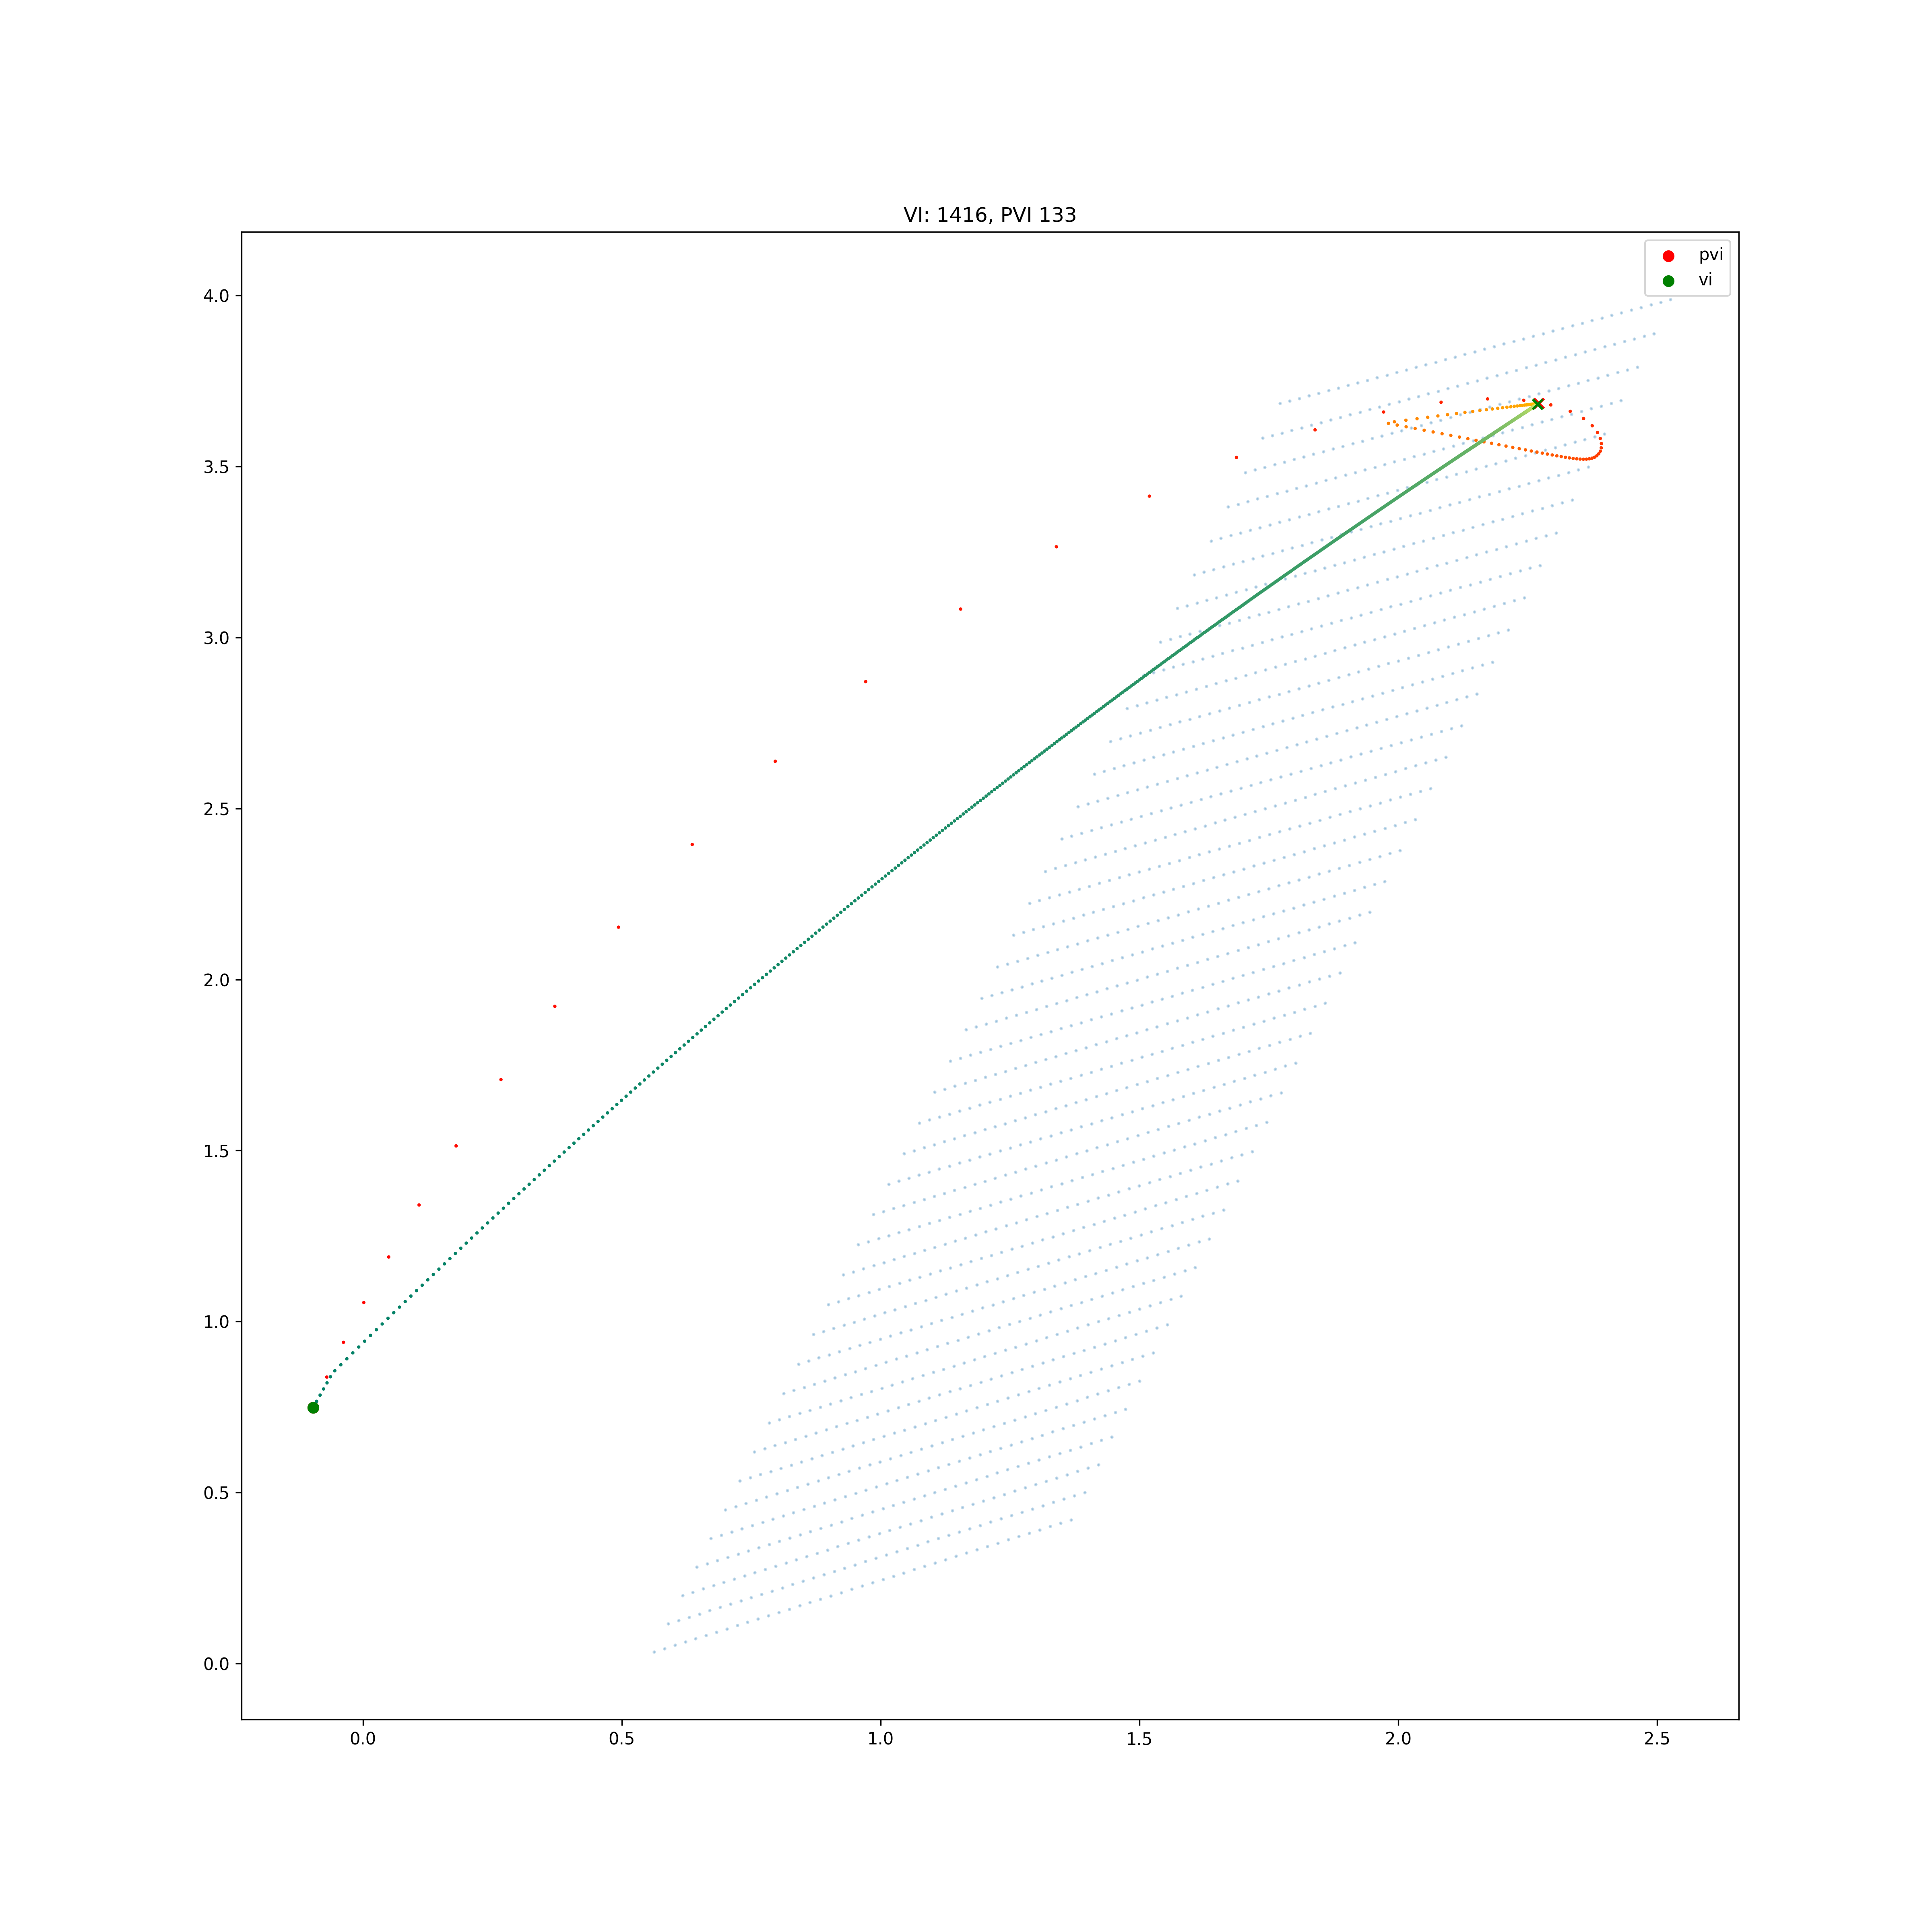
\includegraphics[width=0.5\textwidth,height=0.5\textheight]{../../pictures/figures/vi-vs-pvi.png}
\caption{The optimisation dynamics of value iteration versus parameterised value iteration.}
\end{figure}

\begin{figure}
\centering
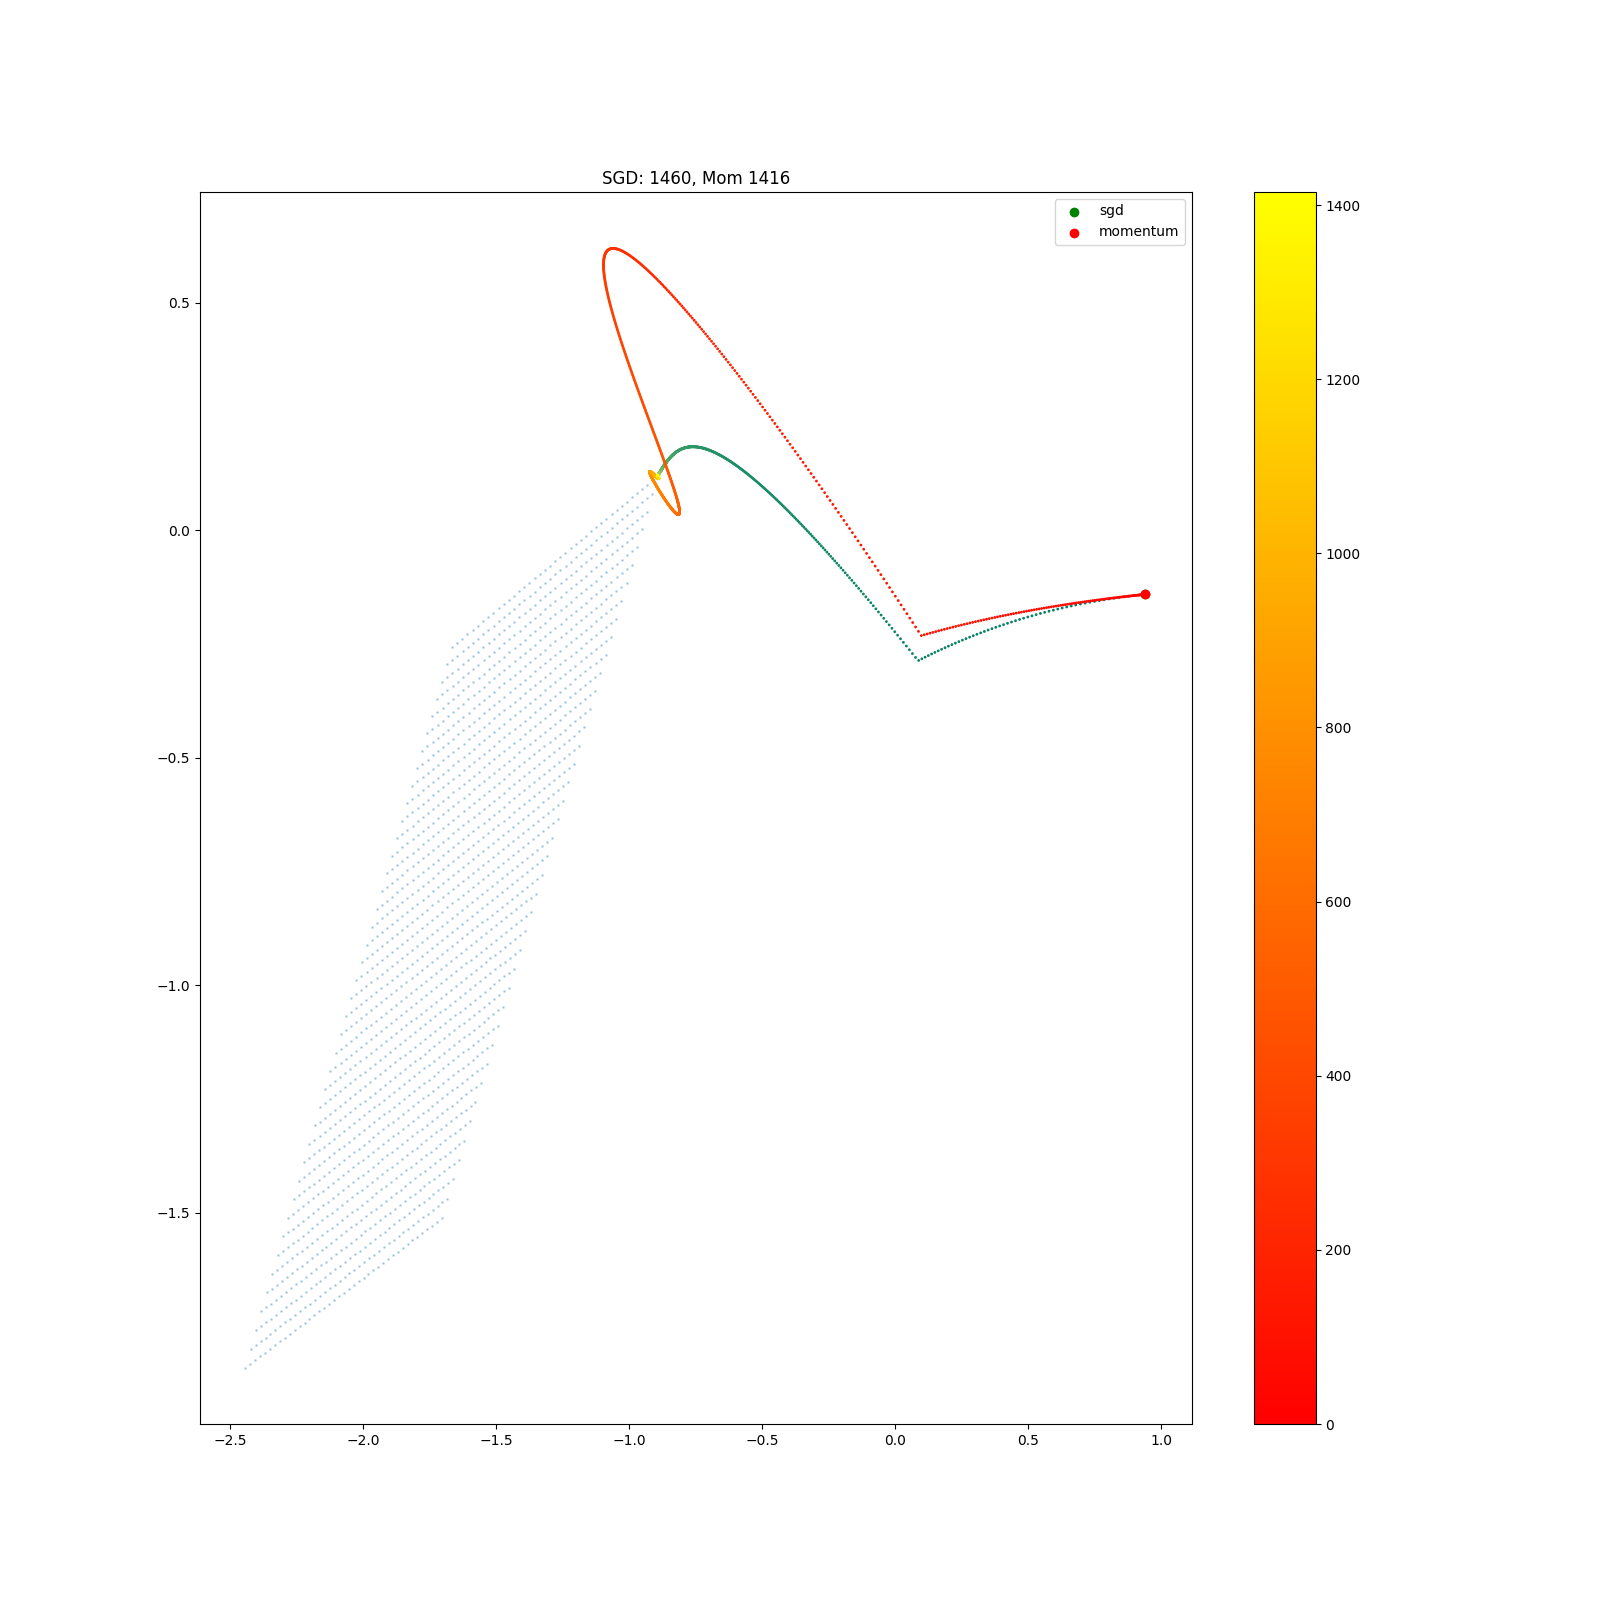
\includegraphics[width=0.5\textwidth,height=0.5\textheight]{../../pictures/figures/vi_sgd-vs-vi_mom.png}
\caption{The optimisation dynamics of value iteration versus value iteration with momentum.}
\end{figure}

If we overparameterise the search space, then we can move between solutions in new ways. We can `tunnel' from A to B, without crossing C.
%  insert pic / prove

Every point (in output space) is closer, when measured in the distance in parameter space needed to be traveled.
% insert pic / prove


\subsection{Acceleration and parameterisation}

{\color{red}insert iteration complexity figures of different lrs with parameterisation.}

\cite{Arora2018} shows that overparameterisation yields acceleration. Consider
the dynamics of the parameter $w$, which we have overparameterised as $w_1 \cdot w_2$.


% Does it even make sense to do a first order approx when trying to reason about momentum?
% Momentum get interesting when considering non-first order factors?!?

We have implicit momentum from the parameterisation, and explicit momentum in the accelerated descent.


\begin{align}
m_{t+1} &= \gamma m_t + g_t \\
w_{t+1} &= w_t - \eta \cdot (1-\gamma) \cdot m_t
\end{align}

It is necessary to consider the trajectory to study momentum. It depends
on what has happened in the past. Can we construct a space of possible
trajectories? What properties do trajectories have? They are connected
by the update fn.


\section{Conclusion}

So, we have seen, from our brief exploration of some properties of MDPs, that
there are some mysteries of interest to the ML community: the optimisation dynamics and generalisation of
parameterised function approximators.
There are unexplored types of solution strategy (???): model iteration. Which might be of interest to

So, while MDPs may be simple, we have yet to fully understand them or explore their ???.

Havent characterised their complexity?!? Sparse, ...

Hopefully we are now prepared to consider how abstraction can be used to improve the efficiency of RL for solving MDPs.



Recently there has been work investigating the properties of overparameterised search spaces.
Many \cite{Arora2018} (and others?!?!?) claim that overparameterisation yeilds acceleration, however,
their explanation of the acceleration is not entirely convincing. Bc...

How does momentum bias the kinds of solution that is converged to. (not really a question for RL?!)
Do we care aout the intermediate policies? In the synchronous setting no. In the asynchronous setting yes.
How does momentum bias trajectories? To cover more distance? To have more diversity?

Search spaces with alternative geometries.
Hyperbolic neural networks. https://arxiv.org/pdf/1805.09112.pdf
